\documentclass[aspectratio=169]{beamer}

\usepackage[utf8]{inputenc}
\usepackage[spanish]{babel}
\usepackage{booktabs}
\usepackage{array}
\usepackage{xcolor}
\usepackage{graphicx}

\usetheme{Madrid}
\usecolortheme{default}

\setbeamertemplate{navigation symbols}{}
\setbeamertemplate{footline}[frame number]

\definecolor{okgreen}{RGB}{34,139,34}
\definecolor{warnorange}{RGB}{204,102,0}
\definecolor{badred}{RGB}{178,34,34}

\title[Detección de Enfermedades en Cultivos]{Sistema Inteligente para la Detección de\\Enfermedades en Cultivos mediante CNN}
\subtitle{Avance del proyecto — Fases de modelado}
\author{Grupo 2}
\date{15 de julio de 2026}

\begin{document}

% ---------------------------------------------------------
\begin{frame}
  \titlepage
\end{frame}

% ---------------------------------------------------------
\begin{frame}{Agenda}
  \tableofcontents
\end{frame}

% ===========================================================
\section{Objetivo y arquitectura}

\begin{frame}{Objetivo del proyecto}
  \begin{itemize}
    \item Construir un sistema capaz de identificar el \textbf{cultivo} y la \textbf{enfermedad} presente en una hoja a partir de una imagen.
    \item Comparar dos enfoques de Deep Learning:
    \begin{itemize}
      \item Una \textbf{CNN propia}, diseñada desde cero.
      \item \textbf{Transfer Learning} con \textbf{ResNet50} preentrenada en ImageNet.
    \end{itemize}
    \item Exponer el mejor modelo mediante una \textbf{API REST (Flask)}, contenida en \textbf{Docker}, con un frontend web para pruebas.
  \end{itemize}
\end{frame}

\begin{frame}{Arquitectura general}
  \begin{itemize}
    \item \textbf{Frontend}: separado en HTML / CSS / JS independientes (antes estaba todo en un solo archivo).
    \item \textbf{API}: Flask, endpoint \texttt{/predict} (recibe imagen, responde cultivo + enfermedad + probabilidad), \texttt{/health}, \texttt{/model/info}.
    \item \textbf{Contenedor}: Dockerfile + \texttt{.dockerignore} propios, con \texttt{HEALTHCHECK}.
    \item \textbf{Modelos}: entrenados en notebooks separados y luego cargados por la API (\texttt{models/*.keras}).
  \end{itemize}
\end{frame}

% ===========================================================
\section{Estrategia de entrenamiento}

\begin{frame}{El reto del tamaño del dataset}
  \begin{block}{Dataset: ``New Plant Diseases Dataset (Augmented)''}
    38 clases (cultivo + enfermedad), aprox. 70{,}295 imágenes de entrenamiento y 17{,}572 de validación.
  \end{block}
  \vspace{0.3cm}
  \begin{alertblock}{Dificultad encontrada}
    El dataset pesa cerca de \textbf{3\,GB}. La descarga local (incluso vía API de Kaggle) resultó extremadamente lenta con nuestra conexión, haciendo inviable el flujo ``descargar $\rightarrow$ entrenar localmente'' dentro de los tiempos del proyecto.
  \end{alertblock}
\end{frame}

\begin{frame}{Decisión: migrar a Kaggle Notebooks}
  \begin{itemize}
    \item Kaggle ofrece GPU gratuita (T4 / P100) y el dataset ya montado en \texttt{/kaggle/input}, \textbf{sin necesidad de descargarlo}.
    \item Se adaptaron los 5 scripts del pipeline (\texttt{scripts/01-06}) a una versión ``Kaggle-ready'' en \texttt{kaggle\_notebook/}.
    \item En paralelo, se preparó también un entorno \textbf{local con GPU} (Miniconda + TensorFlow 2.10.1 + CUDA 11.2 + cuDNN 8.1), para poder repartir carga de entrenamiento entre ambos entornos.
  \end{itemize}
\end{frame}

% ===========================================================
\section{Avance por fases}

\begin{frame}{Resumen de avance}
  \centering
  \begin{tabular}{p{5.2cm}p{3.5cm}}
    \toprule
    \textbf{Fase} & \textbf{Estado} \\
    \midrule
    Fase 1 — Exploración (EDA) & \textcolor{okgreen}{\textbf{Completada}} \\
    Fase 2 — Preprocesamiento y Augmentation & \textcolor{okgreen}{\textbf{Completada}} \\
    Fase 3 — CNN propia & \textcolor{okgreen}{\textbf{Completada}} \\
    Fase 4 — Transfer Learning (ResNet50) & \textcolor{badred}{\textbf{Interrumpida (2 intentos)}} \\
    Fase 5 — Evaluación comparativa & \textcolor{warnorange}{\textbf{Pendiente}} \\
    Docker + despliegue & \textcolor{warnorange}{\textbf{Preparado, sin probar}} \\
    Subida a GitHub & \textcolor{badred}{\textbf{Pendiente}} \\
    \bottomrule
  \end{tabular}
\end{frame}

\begin{frame}{Fase 1 y 2 — EDA y Preprocesamiento}
  \begin{itemize}
    \item Se analizaron las 38 clases: conteo de imágenes, balance entre clases, resolución.
    \item Se generó \texttt{class\_mapping.json}: traduce cada clase técnica (ej. \texttt{Tomato\_\_\_Early\_blight}) a \textit{cultivo} + \textit{enfermedad} en español — pieza clave que usa la API para responder.
    \item Se configuró \textbf{Data Augmentation} (rotación, zoom, brillo, flip horizontal) para mejorar la generalización del modelo.
    \item Reportes y gráficos generados correctamente en \texttt{reports/}.
  \end{itemize}
\end{frame}

\begin{frame}{Fase 1 — EDA: distribución y balance de clases}
  \centering
  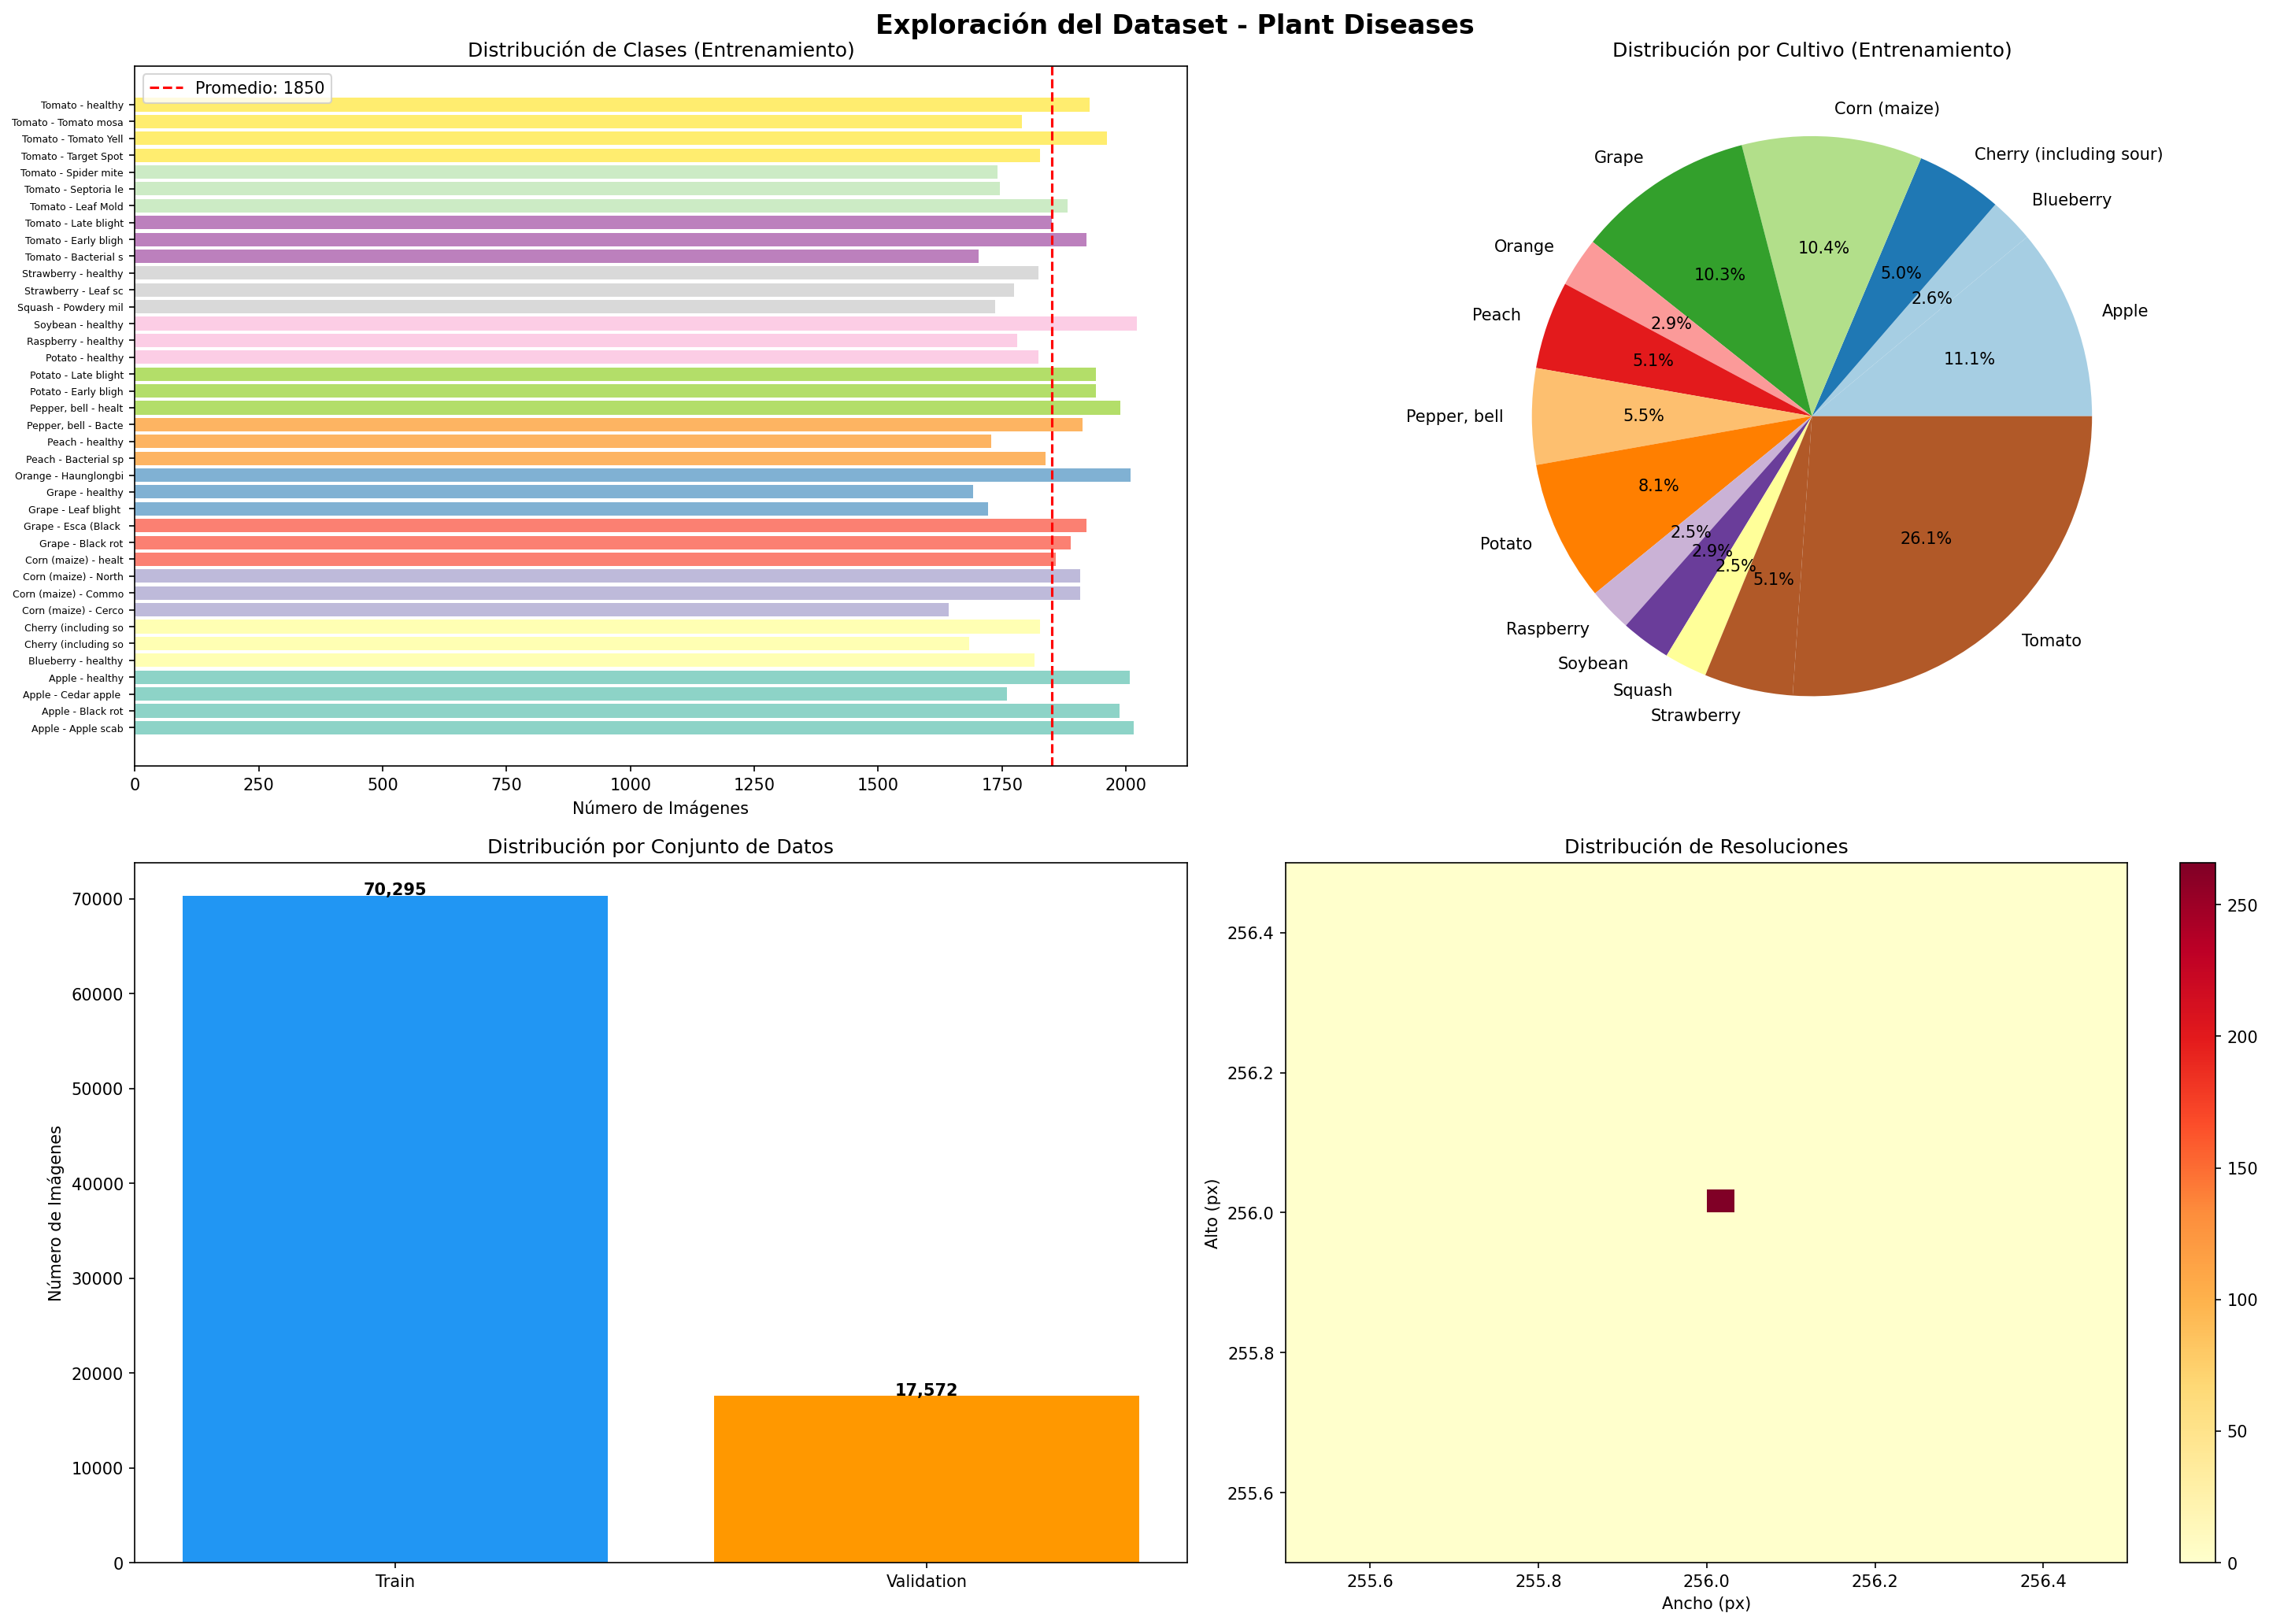
\includegraphics[width=0.85\textwidth]{images/eda_analysis.png}
\end{frame}

\begin{frame}{Fase 2 — Distribución tras el preprocesamiento}
  \centering
  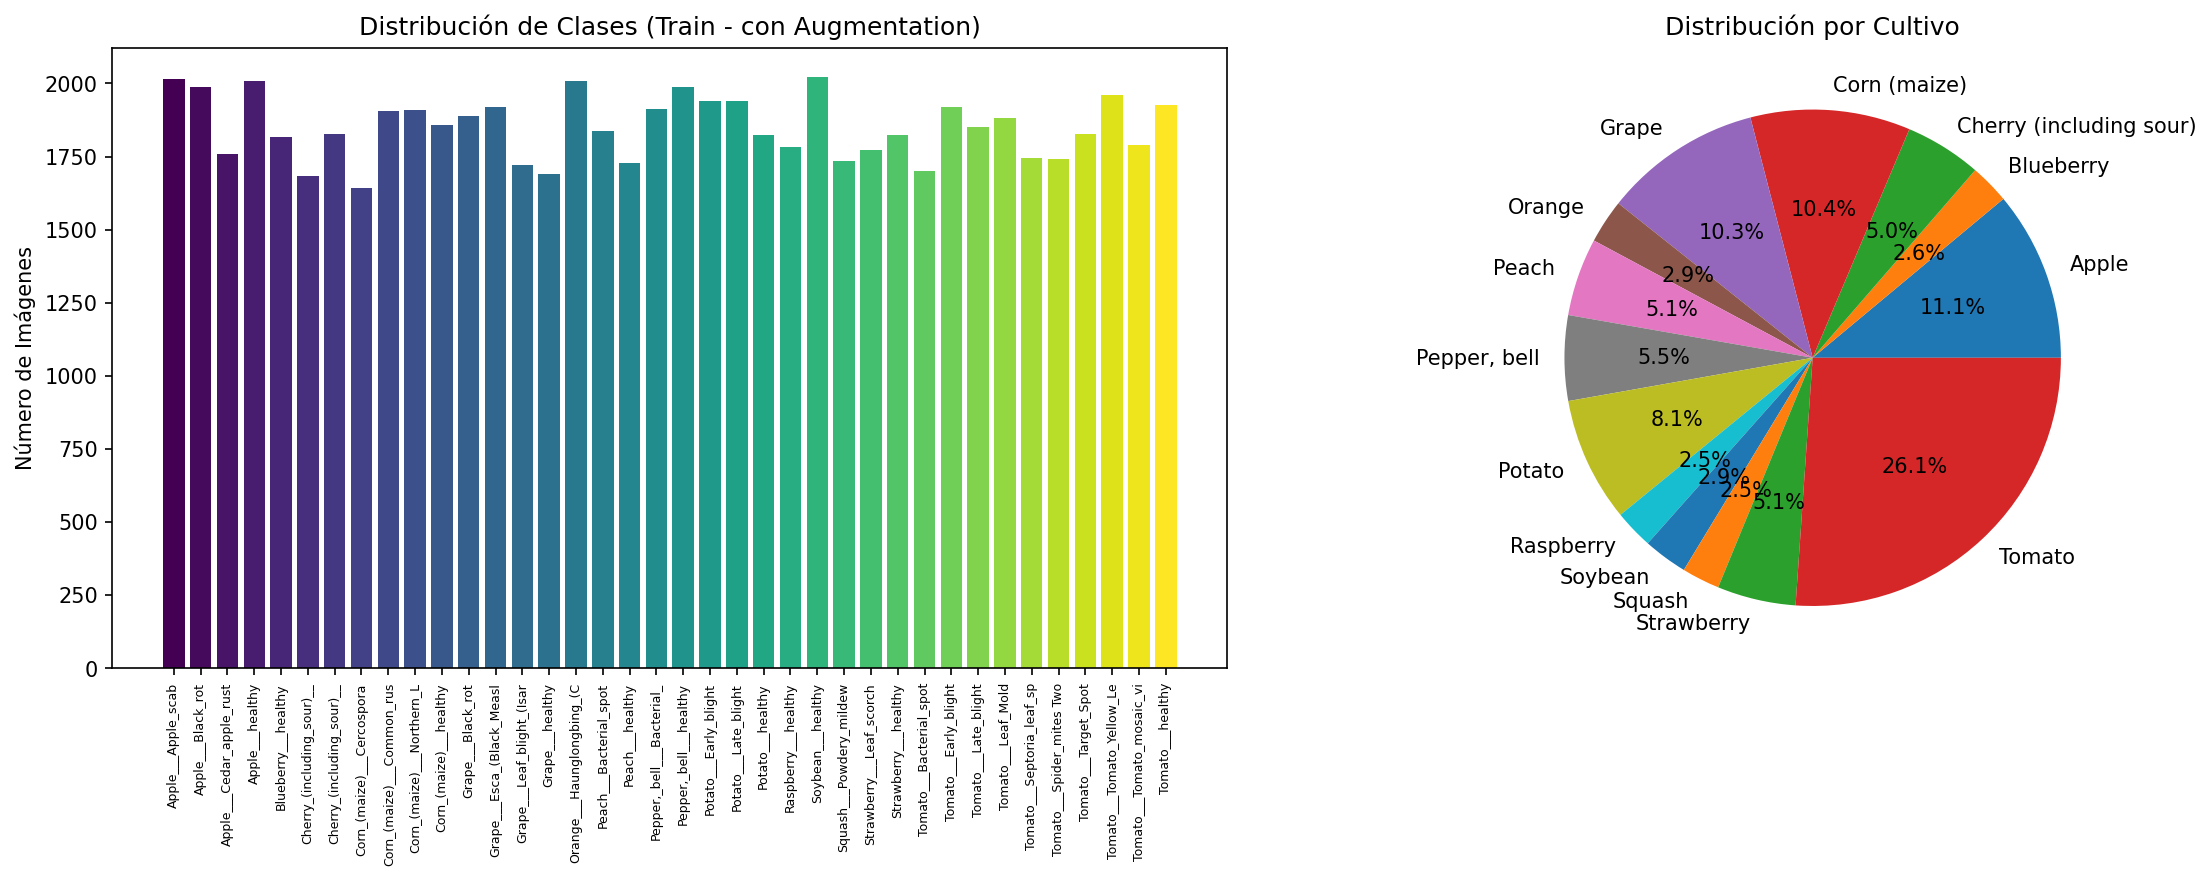
\includegraphics[width=0.72\textwidth]{images/class_distribution_preprocessed.png}
\end{frame}

\begin{frame}{Fase 2 — Ejemplo de Data Augmentation}
  \centering
  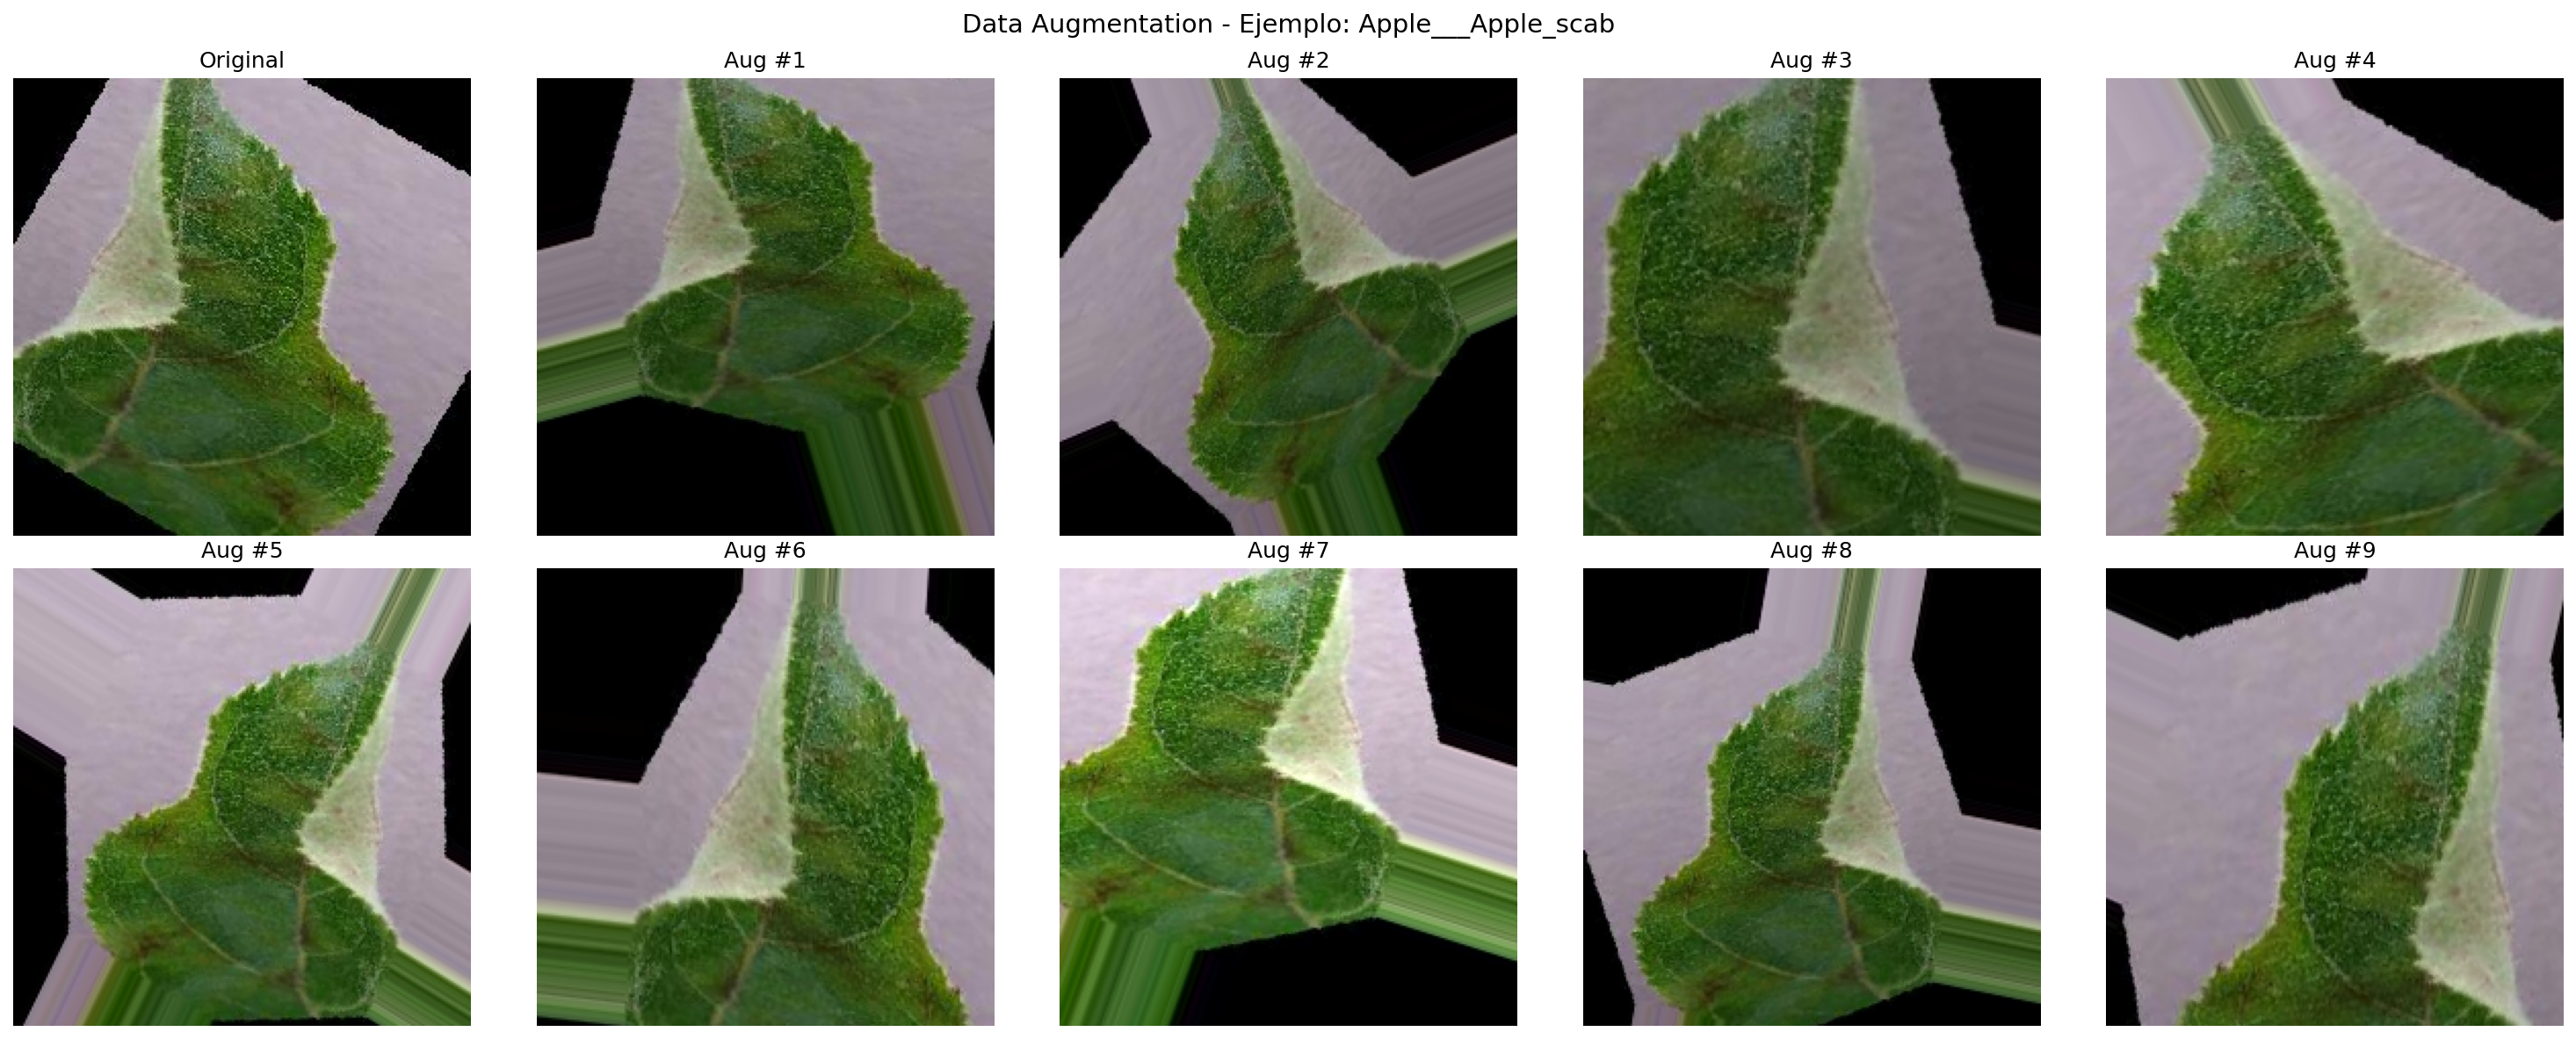
\includegraphics[width=0.78\textwidth]{images/data_augmentation_example.png}
\end{frame}

\begin{frame}{Fase 3 — CNN propia: resultado}
  \begin{block}{Arquitectura}
    4 bloques convolucionales (32 $\to$ 64 $\to$ 128 $\to$ 256 filtros) con BatchNorm y Dropout, sin usar ningún modelo preentrenado.
  \end{block}
  \begin{itemize}
    \item Entrenada en Kaggle mediante \textbf{``Save Version''} (ejecución en segundo plano, no depende de mantener el navegador abierto).
    \item \textbf{Resultado: $\approx$ 99.7\% de accuracy en validación.}
    \item Checkpoint del mejor modelo (\texttt{cnn\_custom\_best.keras}) descargado y ya integrado al proyecto local.
    \item Detalle menor: la sesión de Kaggle se cortó justo después de guardar el mejor checkpoint, por lo que no se generaron el modelo ``final'' ni el JSON de métricas — no es bloqueante, la API solo necesita el ``best''.
  \end{itemize}
\end{frame}

\begin{frame}{Fase 3 — Resultado CNN Propia}
  \centering
  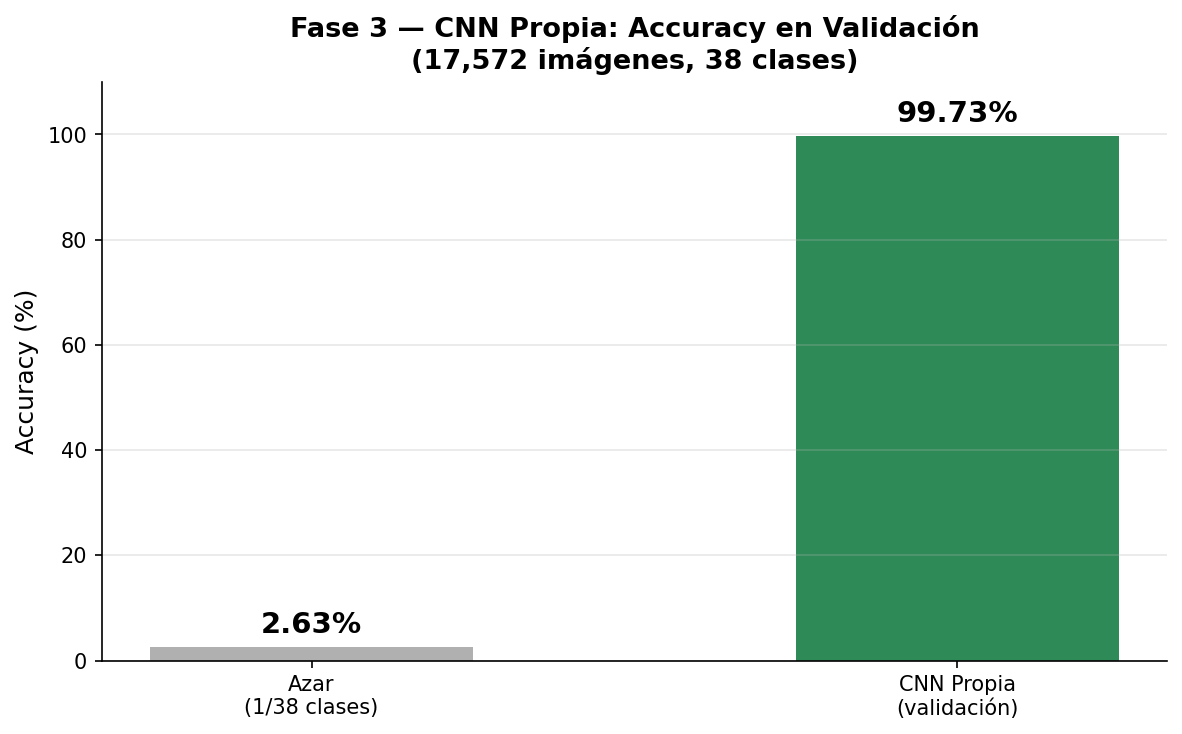
\includegraphics[width=0.68\textwidth]{images/cnn_custom_result.png}
  \vspace{0.3cm}
  \footnotesize Nota: no se generaron las curvas de entrenamiento por época (\texttt{cnn\_custom\_training.png}) porque la sesión de Kaggle se cortó antes de esa etapa final del script; el valor mostrado es el accuracy real del checkpoint guardado.
\end{frame}

% ===========================================================
\section{Fase 4 — ResNet50: qué pasó}

\begin{frame}{Intento 1: entrenamiento local}
  \begin{itemize}
    \item Se lanzó el entrenamiento localmente usando la GPU del equipo (RTX 3050 laptop) con el dataset ya descargado.
    \item El proceso \textbf{se interrumpió antes de terminar} (aprox. 6 horas después de iniciado, sin actividad posterior) — muy probablemente por suspensión del equipo o cierre de la sesión.
    \item Se recuperó únicamente un checkpoint intermedio, guardado automáticamente durante el entrenamiento.
  \end{itemize}
\end{frame}

\begin{frame}{Verificación del checkpoint recuperado}
  \begin{itemize}
    \item Se cargó el checkpoint y se evaluó contra las 17{,}572 imágenes de validación.
  \end{itemize}
  \begin{alertblock}{Resultado de la verificación}
    \textbf{Val Accuracy: 23.9\%} — \quad \textbf{Val Loss: 4.72}
  \end{alertblock}
  \begin{itemize}
    \item Muy por debajo de lo esperado para ResNet50 con transfer learning (normalmente 85–95\%+ en este dataset).
    \item Confirma que el entrenamiento se cortó en una etapa muy temprana. \textbf{El checkpoint no es utilizable.}
  \end{itemize}
\end{frame}

\begin{frame}{Decisión y siguiente intento}
  \begin{itemize}
    \item Dado que el enfoque ``Save Version'' de Kaggle funcionó de forma confiable para la CNN propia (corre en segundo plano, sin depender del navegador ni de la laptop encendida), se decidió repetir el mismo enfoque para ResNet50.
    \item Script \texttt{kaggle\_notebook/04\_transfer\_learning.py} ya ajustado y listo para lanzar.
  \end{itemize}
  \begin{block}{Estimación de tiempo}
    Completar las 30 épocas configuradas para ResNet50 (23M+ parámetros, últimas 30 capas descongeladas, $\sim$70k imágenes de entrenamiento) tomaría aproximadamente \textbf{8 a 10 horas} de cómputo continuo.
  \end{block}
\end{frame}

% ===========================================================
\section{Limitaciones y dificultades}

\begin{frame}{Limitaciones encontradas}
  \begin{itemize}
    \item \textbf{Tamaño del dataset ($\sim$3\,GB)}: la descarga local fue extremadamente lenta, forzando el cambio de estrategia hacia Kaggle.
    \item \textbf{Cuotas de Kaggle}: sesiones gratuitas de GPU limitadas ($\sim$9–12 h por sesión, $\sim$30 h/semana), lo que restringe cuántos reintentos se pueden hacer.
    \item \textbf{Interrupciones de entrenamiento}: tanto local (suspensión del equipo) como en Kaggle (corte de sesión antes de guardar artefactos finales de la CNN).
    \item \textbf{Hardware local limitado}: GPU de laptop (RTX 3050) suficiente para validar checkpoints, pero no ideal para entrenar ResNet50 completo en tiempos cortos.
    \item \textbf{Tiempo de cómputo de ResNet50}: al ser un modelo mucho más pesado que la CNN propia, su entrenamiento completo requiere varias horas, lo que aún está pendiente de completarse.
  \end{itemize}
\end{frame}

% ===========================================================
\section{Próximos pasos}

\begin{frame}{Próximos pasos}
  \begin{enumerate}
    \item Ejecutar Fase 4 (ResNet50) vía Kaggle ``Save Version'' hasta completarla.
    \item Descargar artefactos finales (\texttt{resnet50\_best.keras}, resultados) al repositorio local.
    \item Ejecutar Fase 5: evaluación comparativa (accuracy, precision, recall, F1, matriz de confusión) entre CNN propia y ResNet50.
    \item Probar la API Flask localmente (\texttt{/predict}, \texttt{/health}).
    \item Construir y probar la imagen Docker de extremo a extremo.
    \item Subir el proyecto completo a un repositorio de GitHub.
  \end{enumerate}
\end{frame}

% ---------------------------------------------------------
\begin{frame}
  \centering
  \Large \textbf{¡Gracias!}\\[0.5cm]
  \normalsize Preguntas y comentarios
\end{frame}

\end{document}
